%~~~~~~~~~~~~~~~~~~~~~~~~~~~~~~~~~~~~~~~~~~~~~~~~~~~~~~~~~~~~~~~~~~~~~~~~~~~~~~
% The following are frequently used packages to write an academic paper

\documentclass{article} % set the document class
\usepackage[utf8]{inputenc} % set the encoding
\usepackage{fullpage} % set all page margins to 1.5cm
\usepackage{hyperref} % Produce hypertext links in the document
\usepackage[authoryear, sort]{natbib}  % for nice author-year references
\usepackage{amssymb, amsthm, amsmath} % Packages to write mathematical formulas
\usepackage{cleveref} % in-text references
\usepackage[dvipsnames*,svgnames]{xcolor}% used for font colors
\usepackage{color}% used for background colors
\usepackage{graphicx} % key-value interface for optional arguments to the \includegraphics command
\usepackage[font={sf,small}]{floatrow} % provides many ways to customize layouts of floating environments
\usepackage{paracol} % for multiple columns
\usepackage{booktabs}% fot beautiful tables
\usepackage{caption} % to set font size in captions
    \captionsetup{font=footnotesize}
\usepackage{adjustbox} % to adjust the size of boxes
%~~~~~~~~~~~~~~~~~~~~~~~~~~~~~~~~~~~~~~~~~~~~~~~~~~~~~~~~~~~~~~~~~~~~~~~~~~~~~~

%~~~~~~~~~~~~~~~~~~~~~~~~~~~~~~~~~~~~~~~~~~~~~~~~~~~~~~~~~~~~~~~~~~~~~~~~~~~~~~
% This package is strictly to custom-select hyperlinks' colors and style
\hypersetup{
    colorlinks=true,
    linkcolor = Green,
    urlcolor = Green,
    citecolor = Green
}

\definecolor{azure}{rgb}{0.0, 0.5, 1.0}
%~~~~~~~~~~~~~~~~~~~~~~~~~~~~~~~~~~~~~~~~~~~~~~~~~~~~~~~~~~~~~~~~~~~~~~~~~~~~~~

%~~~~~~~~~~~~~~~~~~~~~~~~~~~~~~~~~~~~~~~~~~~~~~~~~~~~~~~~~~~~~~~~~~~~~~~~~~~~~~
% This package is strictly for verbatim font colors
\usepackage{fancyvrb} 
%~~~~~~~~~~~~~~~~~~~~~~~~~~~~~~~~~~~~~~~~~~~~~~~~~~~~~~~~~~~~~~~~~~~~~~~~~~~~~~

%~~~~~~~~~~~~~~~~~~~~~~~~~~~~~~~~~~~~~~~~~~~~~~~~~~~~~~~~~~~~~~~~~~~~~~~~~~~~~~
% These packages are strictly to add the Overleaf logo to the title
\usepackage[firstpage=true,placement=top,position={14.5,0}]{background}
\backgroundsetup{contents=
\includegraphics{overleaf.png}, scale=1, opacity=0.75}
%~~~~~~~~~~~~~~~~~~~~~~~~~~~~~~~~~~~~~~~~~~~~~~~~~~~~~~~~~~~~~~~~~~~~~~~~~~~~~~

%~~~~~~~~~~~~~~~~~~~~~~~~~~~~~~~~~~~~~~~~~~~~~~~~~~~~~~~~~~~~~~~~~~~~~~~~~~~~~~
% Creating a new environment to put text blocks in a box 
\newenvironment{boxedd}[1]
    {\begin{center}
    #1\\[1ex]
    \begin{tabular}{|p{1\textwidth}|}
    \hline\\
    }
    { 
    \\\\\hline
    \end{tabular} 
    \end{center}
    }
%~~~~~~~~~~~~~~~~~~~~~~~~~~~~~~~~~~~~~~~~~~~~~~~~~~~~~~~~~~~~~~~~~~~~~~~~~~~~~~

%~~~~~~~~~~~~~~~~~~~~~~~~~~~~~~~~~~~~~~~~~~~~~~~~~~~~~~~~~~~~~~~~~~~~~~~~~~~~~~


%~~~~~~~~~~~~~~~~~~~~~~~~~~~~~~~~~~~~~~~~~~~~~~~~~~~~~~~~~~~~~~~~~~~~~~~~~~~~~~

%~~~~~~~~~~~~~~~~~~~~~~~~~~~~~~~~~~~~~~~~~~~~~~~~~~~~~~~~~~~~~~~~~~~~~~~~~~~~~~
% This area, after selecting the document class (first command) and before \begin{document} is called the PREAMBLE. The following commands are always set in the PREABLME area, before the beginning of a document

\title{Gentle introduction to \LaTeX\ and Overleaf }

\author{Michelle González Amador%
    \footnote{UNU-MERIT \& Maastricht University, School of Business and Economics, \href{mailto:mgonzalez@merit.unu.edu}{mgonzalez@merit.unu.edu}}
\and
Paloma de Melo Assunçao%
    \footnote{UNU-MERIT \& Maastricht University, School of Business and Economics, \href{mailto:assuncao@merit.unu.edu}{assuncao@merit.unu.edu}}
}

\date{\today}
%~~~~~~~~~~~~~~~~~~~~~~~~~~~~~~~~~~~~~~~~~~~~~~~~~~~~~~~~~~~~~~~~~~~~~~~~~~~~~~

\begin{document}

\maketitle % This command is necessary to render the \title{} command above

\section{Preliminaries}
\label{section:Preliminaries}

\hyperlink{https://www.latex-project.org/}{\LaTeX{}} is a is a high-quality typesetting system; it includes features designed for the production of technical and scientific documentation. \LaTeX{} is the de facto standard for the communication and publication of scientific documents.
\vspace{1.5em}

\noindent \hyperlink{https://www.overleaf.com/}{Overleaf} is a collaborative cloud-based \LaTeX{} editor used for writing, editing and publishing scientific documents.

\section{Document Structure}
\LaTeX{} allows users to structure their documents with a variety of hierarchical constructs, including chapters, sections, subsections and paragraphs. Given only the logical and semantical structure of a text, \LaTeX{} derives the typographical form of the text according to the “rules” given in the document class (cf. \cref{subsection:documentclass}) and in various style files \citep{baramidze2013latex}. 

\paragraph{Global structure:} When \LaTeX{} processes an input file, it expects it to follow a certain structure. Thus every input file must contain the commands:
\vspace{0.5cm} % this line allows us to select the space between the element above and the one that follows

\begin{figure}[h]
    \centering
    \href{https://en.wikibooks.org/wiki/LaTeX/Document_Structure}{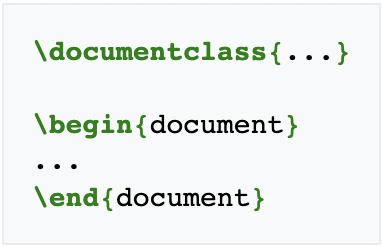
\includegraphics[scale=0.7,]{globalstructure.png}}
    \caption{Global Structure}
    \label{fig:globalstructure}
\end{figure}

\subsection{Document class}
\label{subsection:documentclass}
When processing an input file, \LaTeX{} needs to know which layout standard to use. This is defined within the {\color{Green}{\verb+\documentclass{}+}} command above, and may be a class file input (with \textit{.cls} extension) or a predefined class. In this document, we default to Article class, but there are other options. \Cref{tab:documentclass} gives a brief overview of the most used layout options in \LaTeX{}/Overleaf: 

\begin{table}[h!t]
    \centering
    \begin{tabular}{c l}
    \multicolumn{2}{c}{\textbf{\scalebox{1.2}{Document Classes}}} \vspace{0.5cm} \\
           \hline
         \textbf{Article} & For articles in scientific journals, presentations, short reports, program documentation, invitations.\\
         
         \textbf{Report} & For longer reports containing several chapters, small books, thesis.\\

         \textbf{Books}  & For books.\\

         \textbf{Beamer} & For writing presentations (see \href{https://en.wikibooks.org/wiki/LaTeX/Presentations}{\LaTeX{}/Presentations}).\\
            \hline
    \end{tabular}
    \caption{{\scalebox{0.8}{Popular document classes}}}
    \label{tab:documentclass}
\end{table}

\subsection{Packages}
\label{subsection:packages}
When putting together your document, you may realize that your chosen layout does not have all the formatting options you are used to with word processors. If you want to include graphics, colored text or source code from a file into your document, you need to enhance the capabilities of \LaTeX{}/Overleaf. Such enhancements are called packages, and they should be specified in the preamble of your document -- i.e., between {\color{Green}{\verb+\documentclass{+}}{\color{black}{\ldots}}{\color{Green}{\verb+}+}} and {\color{Green}{\verb+\begin{+}}{\color{black}{document}}{\color{Green}{\verb+}+}} in Figure \ref{fig:globalstructure}. Overleaf uses \TeX{} Live 2021, which provides about 4000 packages. The full list of packages can be found in the \href{https://www.ctan.org/pkg/}{Comprehensive \TeX{} Archive Network}. 

\begin{center}
    \begin{figure}[h]
        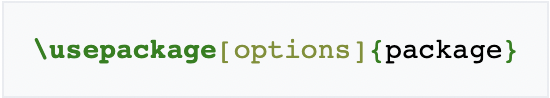
\includegraphics[scale=0.7,]{usepackage.png}
            \caption{Package command line}
            \floatfoot{All packages include options that you can preset before the curly brackets call the desired package.}
        \label{fig:usepackage}
    \end{figure}
\end{center}

At the beginning of this document, you will find that we have selected some basic packages that you can default to when using the most common document classes in \cref{tab:documentclass}, except \textit{beamer}. While these packages are not incompatible with the \textit{beamer} document class, you may benefit more from other packages that are dedicated to illustration and slide design.

\subsection{Document environment}
\label{subsection:environment}
Environments are used to format blocks of text in a \LaTeX{}/Overleaf document. An example of an environment used throughout this document is sectioning (cf. \cref{subsubsection:sectionsandsubs}). Other common environments include centering, lists, equations, and tables. An environment is usually defined within the sequence: \begin{verbatim} \begin{} ...\end{} \end{verbatim}

\paragraph{}
\noindent As a way of illustration, we can create a numbered \& nested list, using the \textsc{enumerate} and \textsc{itemize} environments:

\begin{enumerate}
    \item \LaTeX{}/Overleaf supports the following font features:
        \begin{itemize}
            \item \textbf{bold}
            \item \textit{italic}
        \end{itemize}
    \item \LaTeX{}/Overleaf can be enhanced to include colors:
        \begin{itemize}
            \item {\color{Green} Font colors}
            \item \colorbox{Green}{Background colors}
        \end{itemize}
\end{enumerate}


\subsubsection{Sectioning}
\label{subsubsection:sectionsandsubs}
The commands for inserting sections are fairly intuitive. Of course, certain commands are appropriate to different document classes. For example, a book has chapters but an article doesn't. Sections, subsections, and subsubsections are an essential part of article and report layouts. They are automatically numbered (and ordered). Also, notice that for sections, you do not need to use \verb+\begin{}+ and \verb+\end{}+ commands to indicate which content belongs to a given block.

\paragraph{}
LaTeX provides 7 levels of depth for defining sections (see \cref{tab:sectioning}). Each section in this table is a subsection of the one above it.

\begin{table}[h!t]
    \centering
    \begin{tabular}{l c l}
    \multicolumn{3}{c}{\textbf{\scalebox{1.2}{Sectioning}}} \vspace{0.5cm} \\

           \hline
         \textbf{Command} & \textbf{level} & \textbf{Comment}\\
            \hline
             \verb+\part{}+ & -1 & not in letters\\
             \verb+\chapter{}+ & 0 &	only books and reports\\
             \verb+\section{}+ & 1 & not in letters\\
             \verb+\subsection{}+ & 2 & not in letters\\
             \verb+\subsubsection{}+ & 3 & not in letters\\
             \verb+\paragraph{}+ & 4 & not in letters\\
             \verb+\subparagraph{}+ & 5 & not in letters\\
         
    \end{tabular}
    \caption{Defining sections}
    \label{tab:sectioning}
\end{table}

\subsubsection{Paragraph formatting}
\label{subsubsection:paragraphformat}
\LaTeX{}/Overleaf automatically justifies and indents paragraphs. Should you wish to modify this, you are provided with a series of commands that should be used at the beginning of a paragraph to set your desired style:

\begin{boxedd}{\textbf{Some formatting commands}}
    \begin{itemize}
        \item[ ] \color{Green}{\verb+\raggedright+} \color{black}{for right alignment.}
        \item[ ] \color{Green}{\verb+\raggedleft+} \color{black}{for left alignment.}
        \item[ ] \color{Green}{\verb+\centering+} \color{black}{for centering.}
        \item[ ] \color{Green}{\verb+\indent+} \color{black}{to indent a paragraph that is not indented.}
        \item[ ] \color{Green}{\verb+\indent+} \color{black}{to create a non-indented paragraph.}
        \item[ ] \color{Green}{\verb+\doublespacing+} \color{black}{among other line spacing commands, from the package \color{Green}{\verb+\usepackage{+}\color{black}{setspace}\color{Green}{\verb+}+}}
    \end{itemize}
\end{boxedd}

\paragraph{}
You can also comment out a line, or leave comments in the source code using the \textbf{\%} sign. E.g.:

\begin{center}
 \verb+ \begin{itemize}+ {\color{azure}{\% This command line starts the itemize environment.}}   
\end{center}


\noindent Check the comments in the preamble of this document for more examples. 
\vspace{1em}
There are many other ways in which you can format text and paragraphs that are not covered here, but are easy to find. They are but one Google search away!
\subsubsection{Fonts and Colors}
\label{subsubsection:fontsandcolors}

\columnratio{0.4,0.6}
\begin{paracol}{2}
    \setlength{\columnsep}{2em}
        \begin{leftcolumn}
        
\noindent \underline{\textbf{Some popular fonts:}} \vspace{2mm}
        
\noindent \textrm{Times New Roman}\\
\textsf{Sans Serif}\\
\texttt{Teletype}\\
\textsc{small capitals}
        
        \end{leftcolumn}
% =============================================================================
        \begin{rightcolumn}
        
\noindent \underline{\textbf{Some popular colors:}} \vspace{2mm}
        
\noindent {\color{red}{Red}}\\
{\color{lime}{Lime}}\\
{\color{Green}{\LaTeX{} green}}\\
{\color{azure}{Azure blue}}\\
{\color{magenta}{Magenta}}
        
        \end{rightcolumn}
\end{paracol}

\subsubsection{Labels}
\label{subsubsection:labels}
Every element (table, figure, section, etc.) should be properly labeled using the {\color{Green}{\verb+\label{}+}} command. Labeling does not require an additional package, and it becomes extremely useful to do in-text references (cf. \cref{subsubsection:references}) or easily differentiate an element from another. You'll notice that environments, tables, images and equations have all been labeled throughout this document. 


\subsubsection{In-text references and hyper-references}
\label{subsubsection:references}
To make a reference in text, we recommend the \textit{cleveref} package. \textit{Cleveref} uses labels to redirect the reader to a specific element; i.e.
\color{Green}{\verb+\cref{+}\color{black}{section:Introduction}{\color{Green}{\verb+}+}}. Examples of in-text referencing can be found throughout this document.

\paragraph{}
For hyperlinks, we recommend the \textit{hyperref} package. \textit{Hyperref} is used to handle cross-referencing commands to produce hypertext links in the document. You can use it in text, images, and email addresses. You will find several hypertext links in the document. To learn more about this package, you can go to the \href{https://mirrors.mit.edu/CTAN/macros/latex/contrib/hyperref/doc/hyperref-doc.pdf}{Hyperref Manual}. 

\section{Second-order formatting}
\subsection{Images}
To include images in your document, you'll need the \textit{graphicx} package. The following is an example of how to use the command: 

\begin{center}
    \color{Green}{\verb+\includegraphics+}\color{black}{[scale=1.5]}\color{Green}{\verb+{+}\color{black}{myimage.png}\color{Green}{\verb+}+}
\end{center}

Notice that we have included a scaling parameter in between square brackets. This option allows you to control the size of the image, with 1 being true to size. The image you select must be uploaded as an element in your Overleaf file. You can read more about inserting and positioning images in the \href{https://www.overleaf.com/learn/latex/Inserting_Images}{Overleaf guide} for images.

\begin{figure}[H]
    
\includegraphics[scale=0.3]{latexcoffee.png}
        \label{fig:latexcoffee}
        \caption{\LaTeX{} coffee}
\end{figure}


\subsection{Tables}
Having clean tables goes a long way in making your document look professional. While the default table style provided by \LaTeX{} is not bad, the package \textit{booktabs} offers beautiful typeset tables \citep{fear2005publication}. \Cref{table:MILPtest} is an example of a \textit{booktabs} desgined table:

\begin{table}[h]
\centering
\begin{tabular}{lllllllll}
    \toprule
    \textbf{Budget} & \multicolumn{4}{c}{\textbf{Difference}} & \multicolumn{4}{c}{\textbf{Ratio}}  \\
    \cmidrule(l){2-5}
    \cmidrule(l){6-9}
    & min & max & mean & var & min & max & mean & var \\
    \midrule
    2 & 0.0 & 0.234 & 0.0468 & 0.0109512 & 0.996241 & 1.0 & 0.999248 & 2.82662e-6 \\
    4 & 0.0 & 0.801 & 0.24794 & 0.107615 & 0.992073 & 1.0 & 0.99778 & 1.08092e-5 \\
    6 & 0.1062 & 1.33245 & 0.623518 & 0.386179 & 0.99021 & 0.999471 & 0.996006 & 1.87266e-5 \\
    8 & 0.3413 & 1.31724 & 0.793388 & 0.143545 & 0.993302 & 0.998443 & 0.995982 & 5.22309e-6 \\
    10 & 0.9942 & 1.95934 & 1.48546 & 0.161106 & 0.988431 & 0.995999 & 0.993303 & 8.85753e-6 \\
    12 & 1.1038 & 2.9325 & 2.11843 & 0.494834 & 0.9842 & 0.995961 & 0.991161 & 1.94216e-5 \\
    \bottomrule
\end{tabular}
\caption{Comparison of (non-overlapping) Approximation and Greedy algorithm. For each budget, 10 populations of size $n=250$ are generated with probabilities/utilities drawn uniformly at random from $[1,10]$ and $\{0, 0.1,\ldots, 1 \}$.}
\label{table:MILPtest}
\end{table}

\subsection{Equations}
There are two ways to write an equation. If you want to write a formula in-text, simply use the \textbf{\$} sign. For instance, consider the function 
$f(x)= 3x^3 - 6x^2 + 2x - 1$. Can you find its first derivative? To do so,  we will open an equation environment (from the package \textit{amsmath}): 

\begin{equation}\label{equqation1}
    f'(x) = 9x^2 - 12x + 2
\end{equation}

The equation environment allows you to label, number and subsequently reference the equation in later parts of your document. E.g.: recall equation \eqref{equqation1}, the first derivative of the function $f(x)= 3x^3 - 6x^2 + 2x - 1$.

                                                            \section{Citations and list of references}

In-text citations can be done using packages such as \href{https://www.overleaf.com/learn/latex/Bibliography_management_with_natbib}{natbib}, \href{https://www.overleaf.com/learn/latex/Bibliography_management_with_bibtex}{bibtex} and \href{https://www.overleaf.com/learn/latex/Bibliography_management_with_biblatex}{biblatex}, provided that all your sources are described in a bibliography file (\textit{.bib} extension). These packages are very similar, with differences mostly in citation commands and in citation styles available per package. Here, we use the \textit{abbrvnat} style within the \textit{natbib} package. \vspace{1em}

The bibliography file should provide, for each bibliography entry, a specific set of information such as title, author, and publication year, with more inputs depending on the entry type. \Cref{table:citations} provides some examples of in-text citations, with all sources available in \textit{references.bib}. To create a list of references with \textit{natbib}, simply insert, by the end of your document, the referencing style in {\color{Green}{\verb+\bibliographystyle{+}}{\color{black}{\ldots}}{\color{Green}{\verb+}+}} and the bibliography file name in {\color{Green}{\verb+\bibliography{+}}{\color{black}{\ldots}}{\color{Green}{\verb+}+}}. 

\begin{table}[H]
\centering
\begin{tabular}{ll}
\toprule
Source type & Examples \\
\midrule
Journal articles & \citet{gaudeul2007open}, \citet{baramidze2013latex} \\
Book, book section & \citet{becker1991treatise}, \citet{becker1960economic}\\
Working paper & \citet{bhalotra2010where}\\
\bottomrule
\end{tabular}
\caption{Citation examples}
\label{table:citations}
\end{table}




\newpage % Let's have the resources in a separate page
\section{Helpful resources}
\vspace{2em}

\begin{enumerate}
    \item \TeX{}: Q\&A for users of TeX, LaTeX, ConTeXt, and related typesetting systems. \\
    \vspace{1cm}
         \href{https://tex.stackexchange.com/}{
\includegraphics[scale=0.2]{tex.png}}%
         
    \item \LaTeX{} Wikibook: a guide to the LaTeX typesetting system. It is intended as a useful resource for everybody, from new users who wish to learn, to old hands who need a quick reference.\\
    \vspace{1cm}
        \href{https://en.wikibooks.org/wiki/LaTeX}{
\includegraphics[scale=0.4]{wikibook.png}}%
        
    \item Overleaf tutorials and templates.\\
        \href{https://www.overleaf.com/learn/latex/Tutorials}{
\includegraphics[scale=0.2]{overleaf2.png}}%
    
         
\end{enumerate}

\newpage % we like the reference list/bibliography to start in a new page
%~~~~~~~~~~~~~~~~~~~~~~~~~~~~~~~~~~~~~~~~~~~~~~~~~~~~~~~~~~~~~~~~~~~~~~~~~~~~~~
% Import the bibliography from the .bib file
\bibliographystyle{abbrvnat} % choose the output style of bibliography
\bibliography{references}
%~~~~~~~~~~~~~~~~~~~~~~~~~~~~~~~~~~~~~~~~~~~~~~~~~~~~~~~~~~~~~~~~~~~~~~~~~~~~~~
\end{document}
